\chapter{Planificación}

\section{Seguimiento del desarrollo}
Para el seguimiento y gestión del desarrollo se ha utilizado el software de control de versiones
git\cite{git} en la plataforma Github\cite{Github}.
\\
Se ha creado un github project y se ha utilizado una tabla Kanban para gestionar las historias 
de usuario y las issues del proyecto.
\\\\
El Kanban del proyecto puede verse en el siguiente enlace:
\url{https://github.com/josemip98/TFG/projects/1}

\begin{figure}[!h]
  \centering
  \noindent\makebox[\textwidth]{
    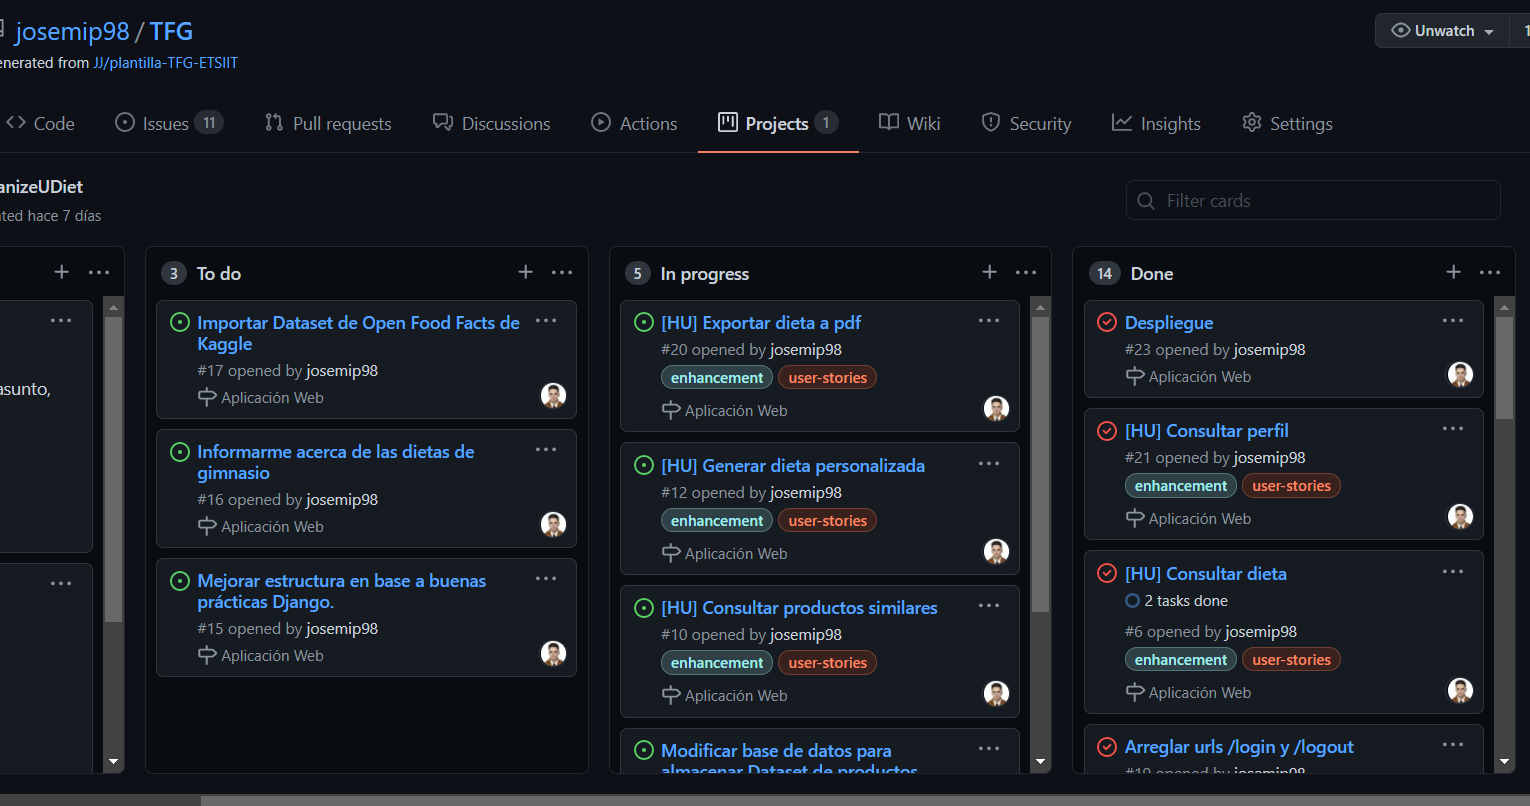
\includegraphics[scale=0.4]{kanban.png}}
  \caption{Tabla Kanban del proyecto.}
\end{figure}

\subsection{Historia de usuario}\label{subsec:hu}
Una historia de usuario es \textbf{una funcionalidad que el usuario espera}.
El modelo a seguir para la creación de historias de usuario es:
\\ \textit{Como usuario/desarrollador quiero poder [funcionalidad] para [razón dicha funcionalidad].}\\

Además podemos añadir tareas que necesitamos cumplir para completar la historia de usuario o detalles técnicos.

\begin{figure}[H]
	\centering	
	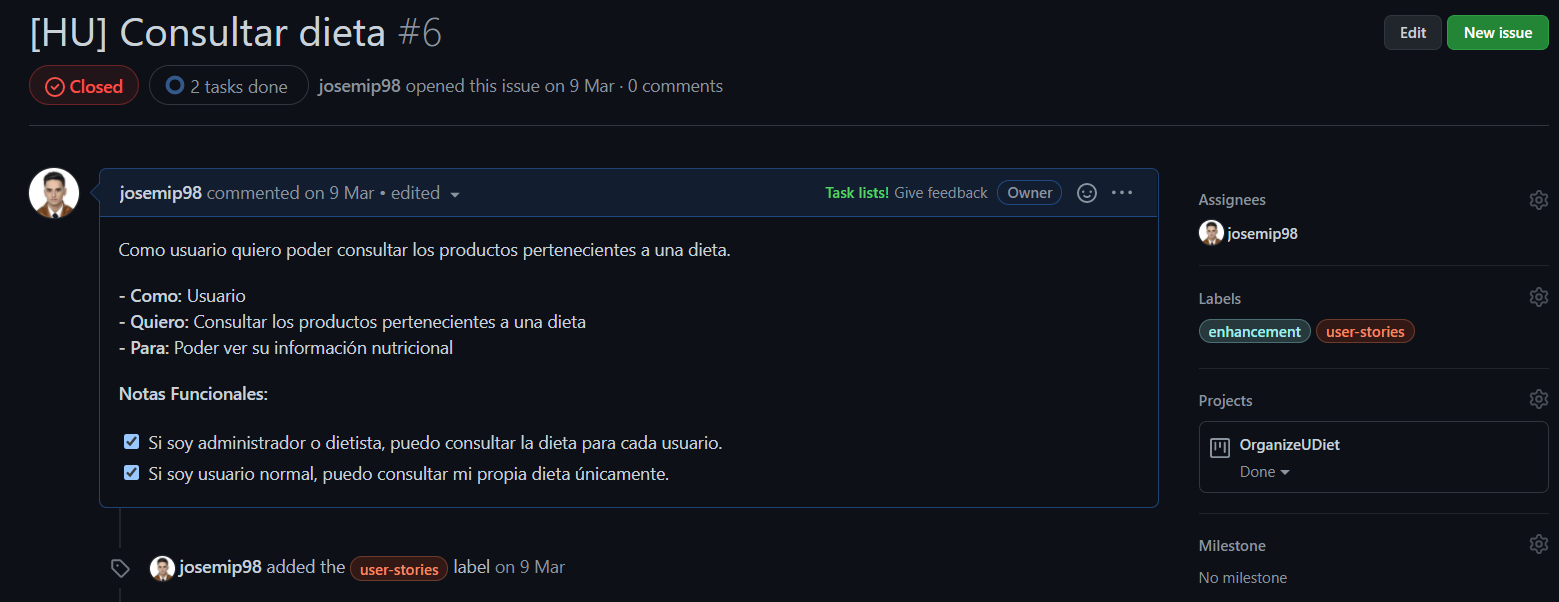
\includegraphics[scale=0.4]{hu.png}
	\end{figure}

\subsection{Issues}\label{subsec:issue}
Las issues pueden ser correción de bugs, mantenimiento del proyecto o tareas que sean necesarias para el desarrollo del proyecto.

\begin{figure}[H]
	\centering	
	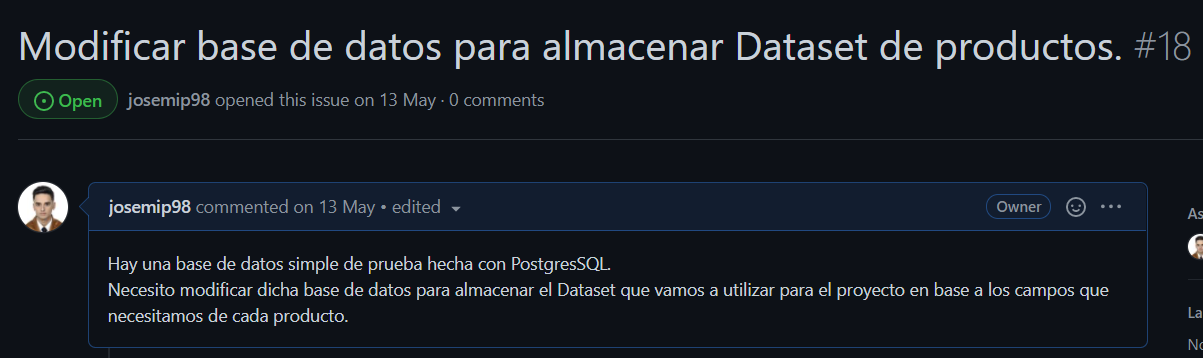
\includegraphics[scale=0.4]{issue.png}
	\end{figure}

\section{Metodología utilizada}

